\documentclass[a4paper,11pt]{article}
\usepackage[utf8]{inputenc}
\usepackage[T1]{fontenc}
\usepackage{amsmath,amssymb}
\usepackage[a4paper,left=2cm,right=2cm,top=3.6cm,bottom=2.3cm,headheight=1.1cm,headsep=0.6cm,footskip=1cm]{geometry}
\usepackage{xcolor}
\usepackage{tikz}
\usetikzlibrary{calc,arrows.meta,positioning,shapes.geometric}
\usepackage{fancyhdr}
\usepackage{lastpage}
\usepackage{tabularx}
\usepackage{array}
\usepackage[most]{tcolorbox}
\usepackage{enumitem}
\usepackage{needspace}

% ---------- palet merah dan merah muda ----------
\definecolor{redx}{HTML}{B3202F}
\definecolor{pinkx}{HTML}{E0457B}
\definecolor{maroon}{HTML}{7A1C2C}
\definecolor{softbg}{HTML}{FDF1F4}
\definecolor{salmon}{HTML}{E8836F}
\newcommand{\dis}{\displaystyle}
\newcommand{\Df}{D_f}
\newcommand{\Rf}{R_f}

\setlength{\parindent}{0pt}
\renewcommand{\arraystretch}{1.35}

\tikzset{
  ov/.style={draw=gray,thick,ellipse,fill=softbg,inner sep=0pt},
  dr/.style={circle,draw=redx,fill=redx!12,minimum size=0.46cm,inner sep=0pt,font=\scriptsize},
  dk/.style={circle,draw=pinkx,fill=pinkx!15,minimum size=0.46cm,inner sep=0pt,font=\scriptsize},
  ar/.style={-{Stealth[length=1.8mm]},thick,redx},
  arp/.style={-{Stealth[length=1.8mm]},thick,pinkx},
  box/.style={draw=redx,thick,rounded corners=3pt,fill=softbg,align=center,inner sep=4pt}
}

% ---------- header berwarna merah ----------
\pagestyle{fancy}
\fancyhf{}
\renewcommand{\headrulewidth}{0pt}
\fancyhead[L]{%
  \begin{tikzpicture}[remember picture,overlay]
    \fill[redx] ([yshift=-1.2cm]current page.north west) rectangle ([yshift=-3.15cm]current page.north east);
    \fill[pinkx] ([yshift=-3.15cm]current page.north west) rectangle ([yshift=-3.25cm]current page.north east);
  \end{tikzpicture}%
  \color{white}\bfseries\large Latihan Soal Komposisi Fungsi dan Invers}
\fancyhead[R]{\color{white}\small Diunduh dari website \textbf{Math1729}\ \,|\,\ 4 Oktober 2026}
\fancyfoot[L]{\small\color{redx}Math1729 --- Komposisi Fungsi dan Invers}
\fancyfoot[R]{\small\color{redx}Halaman \thepage\ dari \pageref{LastPage}}

% ---------- komponen ----------
\newcounter{no}
\newcommand{\bagian}[2]{\par\Needspace{6\baselineskip}\vspace{1.0em}\noindent
  \begin{tcolorbox}[colback=redx,colframe=redx,coltext=white,boxrule=0pt,arc=2pt,left=6pt,right=6pt,top=3pt,bottom=3pt]
  \textbf{#1}\hfill{\small #2}\end{tcolorbox}\setcounter{no}{0}\par\vspace{-0.3em}}
\newcommand{\tingkat}[2]{\par\Needspace{7\baselineskip}\vspace{0.6em}\noindent
  {\color{pinkx}\rule{3pt}{1.1em}}\ {\color{redx}\bfseries #1}\ {\small\color{gray}--- #2}\par\vspace{0.1em}}
\newcommand{\soal}[2]{\par\vspace{0.75em}\stepcounter{no}\noindent
  \begin{minipage}[t]{1.8em}\textbf{\theno.}\end{minipage}%
  \begin{minipage}[t]{\dimexpr\linewidth-1.8em\relax}#1\par\vspace{0.35em}#2\end{minipage}\par}
\newcommand{\poin}[1]{\hfill{\small\color{redx}[#1 poin]}}

% teks di kiri, gambar di kanan
\newcommand{\gbr}[2]{\noindent\begin{minipage}[t]{0.56\linewidth}#1\end{minipage}\hfill\raisebox{\ht\strutbox}{\begin{minipage}[t]{0.41\linewidth}\vspace{0pt}\centering#2\end{minipage}}}

% pilihan jawaban
\newcommand{\pil}[5]{\begin{tabularx}{\linewidth}{@{}*{5}{X}@{}}\textbf{A.}\;#1 & \textbf{B.}\;#2 & \textbf{C.}\;#3 & \textbf{D.}\;#4 & \textbf{E.}\;#5\end{tabularx}}
\newcommand{\pilx}[5]{\begin{tabularx}{\linewidth}{@{}*{3}{X}@{}}\textbf{A.}\;#1 & \textbf{B.}\;#2 & \textbf{C.}\;#3\\[10pt] \textbf{D.}\;#4 & \textbf{E.}\;#5 & \end{tabularx}}
\newcommand{\jwb}{\hfill Jawaban: \rule{4.5cm}{0.4pt}}

\begin{document}
\thispagestyle{fancy}

\begin{center}
  {\color{redx}\fontsize{22}{26}\selectfont\bfseries Latihan Soal Komposisi Fungsi dan Invers\par}
  \vspace{2pt}
  {\color{pinkx}\large Fungsi, Komposisi, Fungsi Invers, dan Invers dari Komposisi\par}
\end{center}
\vspace{2pt}
\begin{tcolorbox}[colback=softbg,colframe=redx!40,boxrule=0.6pt,arc=3pt,left=8pt,right=8pt,top=5pt,bottom=5pt]
\noindent\textbf{Nama} : \rule{4.6cm}{0.4pt}\hfill\textbf{Kelas} : \rule{2.2cm}{0.4pt}\hfill\textbf{Skor} : \rule{2.2cm}{0.4pt}
\end{tcolorbox}
\vspace{2pt}
\begin{tcolorbox}[colback=white,colframe=pinkx,boxrule=0.8pt,arc=3pt,left=8pt,right=8pt,top=4pt,bottom=4pt,title={\bfseries Petunjuk Pengerjaan},coltitle=white,fonttitle=\small]
\small
\begin{enumerate}[leftmargin=1.4em,itemsep=1pt,topsep=1pt]
\item Soal terdiri atas \textbf{20 pilihan ganda} (5 mudah, 5 sedang, 5 sulit, 5 HOTS), \textbf{5 isian singkat}, dan \textbf{5 uraian (essay)}. Soal disusun berjenjang dari mudah sampai HOTS dan sebagian bergaya UTBK. Alokasi waktu yang disarankan: 120 menit.
\item Skor: pilihan ganda 2 poin, isian singkat 4 poin, uraian 8 poin per soal (total 100 poin). Tidak ada pengurangan skor untuk jawaban salah.
\item Notasi: $D_f$ domain, $R_f$ range, $(f\circ g)(x)=f\big(g(x)\big)$, $f^{-1}$ fungsi invers dari $f$, dan $f^{(n)}$ komposisi $f$ sebanyak $n$ kali. Jika domain tidak disebutkan, gunakan domain natural (himpunan bilangan real terbesar yang membuat rumus bermakna). Gambar tidak selalu digambar sesuai skala.
\item Bilangan desimal ditulis dengan tanda koma. Jika perlu, bulatkan hasil sampai dua angka desimal.
\item Kalkulator tidak diperkenankan.
\end{enumerate}
\end{tcolorbox}

% =====================================================================
\bagian{A. Pilihan Ganda}{20 soal $\times$ 2 poin = 40 poin. Pilih satu jawaban yang paling tepat.}

\tingkat{Tingkat Mudah}{soal 1 sampai 5}
\soal{Diketahui $f(x)=3x-2$ dan $g(x)=x^2+1$. Nilai $(g\circ f)(2)$ adalah \dots.}{\pil{$10$}{$13$}{$15$}{$17$}{$20$}}
\soal{\gbr{Diagram panah pada gambar menunjukkan fungsi $f:A\to B$ dan $g:B\to C$. Range dari fungsi $g\circ f$ adalah \dots.}{%
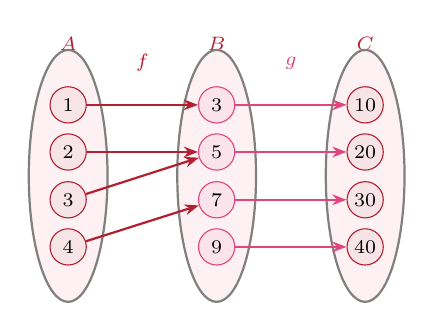
\begin{tikzpicture}[scale=0.82]
\node[font=\scriptsize\bfseries,redx] at (0,2.05) {$A$};
\node[font=\scriptsize\bfseries,redx] at (2.3,2.05) {$B$};
\node[font=\scriptsize\bfseries,redx] at (4.6,2.05) {$C$};
\node[ov,minimum width=1.0cm,minimum height=3.2cm] at (0,0) {};
\node[ov,minimum width=1.0cm,minimum height=3.2cm] at (2.3,0) {};
\node[ov,minimum width=1.0cm,minimum height=3.2cm] at (4.6,0) {};
\foreach \yy/\l in {1.1/1,0.37/2,-0.37/3,-1.1/4}{\node[dr] (a\l) at (0,\yy) {\l};}
\foreach \yy/\l/\v in {1.1/1/3,0.37/2/5,-0.37/3/7,-1.1/4/9}{\node[dk] (b\l) at (2.3,\yy) {\v};}
\foreach \yy/\l/\v in {1.1/1/10,0.37/2/20,-0.37/3/30,-1.1/4/40}{\node[dr] (c\l) at (4.6,\yy) {\v};}
\foreach \i/\j in {1/1,2/2,3/2,4/3}{\draw[ar] (a\i)--(b\j);}
\foreach \i/\j in {1/1,2/2,3/3,4/4}{\draw[arp] (b\i)--(c\j);}
\node[font=\scriptsize,redx] at (1.15,1.75) {$f$};
\node[font=\scriptsize,pinkx] at (3.45,1.75) {$g$};
\end{tikzpicture}}}{\begin{tabularx}{\linewidth}{@{}*{3}{X}@{}}\textbf{A.}\;$\{10,20\}$ & \textbf{B.}\;$\{10,20,30\}$ & \textbf{C.}\;$\{10,20,30,40\}$\\[3pt] \textbf{D.}\;$\{3,5,7\}$ & \textbf{E.}\;$\{3,5,7,9\}$ & \end{tabularx}}
\soal{Diketahui $f(x)=3x-6$. Jika $f^{-1}$ adalah invers dari $f$, nilai $f^{-1}(9)$ adalah \dots.}{\pil{$1$}{$3$}{$5$}{$7$}{$21$}}
\soal{\gbr{Tabel di samping menyajikan nilai fungsi $f$ dan $g$ pada himpunan $\{1,2,3,4\}$. Nilai $(f\circ g)(2)+(g\circ f)(4)$ adalah \dots.}{%
\small
\begin{tabular}{@{}c|cccc@{}}
\hline
$x$ & $1$ & $2$ & $3$ & $4$\\ \hline
$f(x)$ & $3$ & $1$ & $4$ & $2$\\
$g(x)$ & $4$ & $1$ & $2$ & $3$\\ \hline
\end{tabular}}}{\pil{$4$}{$5$}{$6$}{$7$}{$8$}}
\soal{Diketahui $f(x)=x+2$ dan $g(x)=3x-1$. Rumus fungsi $(g\circ f)(x)$ adalah \dots.}{\pil{$3x-1$}{$3x+1$}{$3x+2$}{$3x+3$}{$3x+5$}}

\tingkat{Tingkat Sedang}{soal 6 sampai 10}
\soal{Diketahui $f(x)=2x+1$ dan $(f\circ g)(x)=6x-5$. Fungsi $g(x)$ adalah \dots.}{\pil{$3x-5$}{$3x-\frac{7}{2}$}{$3x-3$}{$6x-6$}{$6x-4$}}
\soal{Diketahui $g(x)=x-2$ dan $(f\circ g)(x)=x^2-4x+5$. Nilai $f(5)$ adalah \dots.}{\pil{$10$}{$26$}{$30$}{$37$}{$50$}}
\soal{Invers dari fungsi $f(x)=\dis\frac{3x-1}{x+2}$, $x\neq-2$, adalah $f^{-1}(x)=\dots$.}{\pilx{$\dis\frac{2x+1}{3-x}$}{$\dis\frac{2x+1}{x-3}$}{$\dis\frac{x+2}{3x-1}$}{$\dis\frac{2x-1}{x+3}$}{$\dis\frac{3x-1}{x+2}$}}
\soal{\gbr{Grafik fungsi linear $f$ pada gambar melalui titik $(1,-1)$ dan $(3,3)$. Jika $f^{-1}$ adalah invers dari $f$, nilai $f^{-1}(7)$ adalah \dots.}{%
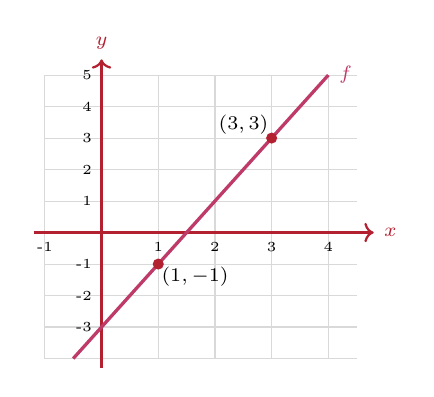
\begin{tikzpicture}[x=0.72cm,y=0.4cm]
\draw[gray!30,xstep=1,ystep=1] (-1,-4) grid (4.5,5);
\draw[->,thick,redx] (-1.2,0)--(4.8,0) node[right,font=\scriptsize]{$x$};
\draw[->,thick,redx] (0,-4.3)--(0,5.5) node[above,font=\scriptsize]{$y$};
\foreach \xx in {-1,1,2,3,4}{\node[below,font=\tiny] at (\xx,0) {\xx};}
\foreach \yy in {-3,-2,-1,1,2,3,4,5}{\node[left,font=\tiny] at (0,\yy) {\yy};}
\draw[pinkx!85!black,very thick] (-0.5,-4)--(4,5) node[right,font=\scriptsize]{$f$};
\fill[redx] (1,-1) circle (2pt) (3,3) circle (2pt);
\node[font=\scriptsize,below right,inner sep=1pt] at (1,-1) {$(1,-1)$};
\node[font=\scriptsize,above left,inner sep=1pt] at (3,3) {$(3,3)$};
\end{tikzpicture}}}{\pil{$2$}{$3{,}5$}{$4$}{$5$}{$11$}}
\soal{Diketahui $f(x)=\sqrt{x}$ dan $g(x)=x^2-4x+3$. Domain dari fungsi $(f\circ g)(x)$ adalah \dots.}{\begin{tabularx}{\linewidth}{@{}*{3}{X}@{}}\textbf{A.}\;$1\le x\le3$ & \textbf{B.}\;$x<1$ atau $x>3$ & \textbf{C.}\;$x\ge3$\\[3pt] \textbf{D.}\;$x\le3$ & \textbf{E.}\;$x\le1$ atau $x\ge3$ & \end{tabularx}}

\tingkat{Tingkat Sulit}{soal 11 sampai 15, setara UTBK}
\soal{Diketahui $f(x)=2x-3$ dan $g(x)=\dis\frac{x+1}{x-2}$, $x\neq2$. Nilai $(f\circ g)^{-1}(3)$ adalah \dots.}{\pil{$3$}{$\frac{13}{4}$}{$\frac{7}{2}$}{$4$}{$\frac{9}{2}$}}
\soal{\gbr{Gambar menunjukkan grafik fungsi $f(x)=x^2-4x+1$ dengan domain $\{x\mid x\ge2\}$ (bagian yang tebal). Jika $f^{-1}$ adalah invers dari $f$, nilai $f^{-1}(6)$ adalah \dots.}{%
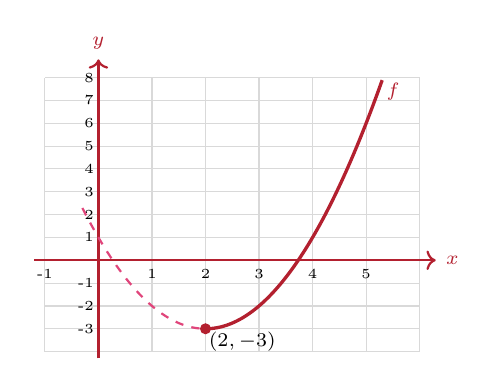
\begin{tikzpicture}[x=0.68cm,y=0.29cm]
\draw[gray!30,xstep=1,ystep=1] (-1,-4) grid (6,8);
\draw[->,thick,redx] (-1.2,0)--(6.3,0) node[right,font=\scriptsize]{$x$};
\draw[->,thick,redx] (0,-4.3)--(0,8.8) node[above,font=\scriptsize]{$y$};
\foreach \xx in {-1,1,2,3,4,5}{\node[below,font=\tiny] at (\xx,0) {\xx};}
\foreach \yy in {-3,-2,-1,1,2,3,4,5,6,7,8}{\node[left,font=\tiny,inner sep=1.5pt] at (0,\yy) {\yy};}
\draw[pinkx,thick,dashed,domain=-0.3:2,samples=30,smooth] plot (\x,{\x*\x-4*\x+1});
\draw[redx,very thick,domain=2:5.3,samples=40,smooth] plot (\x,{\x*\x-4*\x+1});
\fill[redx] (2,-3) circle (2pt);
\node[font=\scriptsize,below right,inner sep=1pt] at (2,-3) {$(2,-3)$};
\node[font=\scriptsize,redx,right] at (5.2,7.4) {$f$};
\end{tikzpicture}}}{\pil{$-1$}{$3$}{$2+\sqrt{6}$}{$5$}{$7$}}
\soal{Fungsi $f(x)=ax+b$ dengan $a>0$ memenuhi $(f\circ f)(x)=4x+9$ untuk setiap bilangan real $x$. Nilai $f^{-1}(11)$ adalah \dots.}{\pil{$2$}{$4$}{$7$}{$9$}{$25$}}
\soal{Diketahui $f(x)=x^2-1$ dan $g(x)=2x+1$ dengan domain semua bilangan real. Perhatikan pernyataan berikut.
\begin{enumerate}[label=(\arabic*),leftmargin=1.8em,itemsep=0pt,topsep=2pt]
\item $(g\circ f)(x)=2x^2-1$.
\item $(f\circ g)(x)=4x^2+4x$.
\item Fungsi $f$ tidak memiliki fungsi invers pada himpunan bilangan real.
\item $(g^{-1}\circ f)(2)=2$.
\end{enumerate}
Pernyataan yang benar adalah \dots.}{\begin{tabularx}{\linewidth}{@{}*{3}{X}@{}}\textbf{A.}\;(1), (2), dan (3) saja & \textbf{B.}\;(1) dan (3) saja & \textbf{C.}\;(2) dan (4) saja\\[3pt] \textbf{D.}\;(4) saja & \textbf{E.}\;(1), (2), (3), dan (4) & \end{tabularx}}
\soal{Di sebuah toko sepatu, kasir menghitung harga pembayaran dengan tiga langkah berurutan seperti pada diagram. Rani membayar Rp132.000 untuk sepasang sepatu. Harga awal sepatu tersebut adalah \dots.
\begin{center}
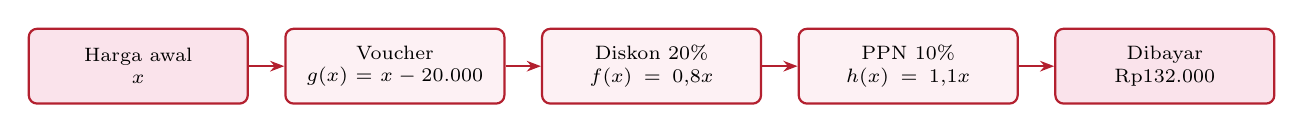
\begin{tikzpicture}[font=\scriptsize,bx/.style={box,text width=2.5cm,minimum height=0.95cm}]
\node[bx,fill=pinkx!15] (a) {Harga awal\\$x$};
\node[bx,right=0.45cm of a] (b) {Voucher\\$g(x)=x-20.000$};
\node[bx,right=0.45cm of b] (c) {Diskon $20\%$\\$f(x)=0{,}8x$};
\node[bx,right=0.45cm of c] (d) {PPN $10\%$\\$h(x)=1{,}1x$};
\node[bx,fill=pinkx!15,right=0.45cm of d] (e) {Dibayar\\Rp132.000};
\foreach \p/\q in {a/b,b/c,c/d,d/e}{\draw[ar] (\p)--(\q);}
\end{tikzpicture}
\end{center}}{\begin{tabularx}{\linewidth}{@{}*{5}{X}@{}}\textbf{A.}\;Rp160.000 & \textbf{B.}\;Rp165.000 & \textbf{C.}\;Rp170.000 & \textbf{D.}\;Rp175.000 & \textbf{E.}\;Rp180.000\end{tabularx}}

\tingkat{Tingkat HOTS}{soal 16 sampai 20, penalaran tingkat tinggi gaya UTBK}
\soal{Diketahui $f(x)=\dis\frac{x+1}{x-1}$, $x\neq1$. Jika $f^{(n)}$ menyatakan komposisi $f$ sebanyak $n$ kali, yaitu $f^{(1)}=f$ dan $f^{(n)}=f\circ f^{(n-1)}$, nilai $f^{(2027)}\!\left(\dis\frac32\right)$ adalah \dots.}{\pil{$1$}{$\frac{3}{2}$}{$\frac{5}{2}$}{$3$}{$5$}}
\soal{Diketahui $f(x)=\dis\frac{ax+b}{2x-3}$, $x\neq\dis\frac32$. Jika $f^{-1}(x)=f(x)$ untuk setiap $x$ dalam domainnya dan $f(2)=5$, nilai $a+b$ adalah \dots.}{\pil{$0$}{$2$}{$4$}{$5$}{$8$}}
\soal{\gbr{Gambar menunjukkan grafik fungsi bijektif $f:[0,6]\to[1,10]$ yang berupa garis patah dengan titik-titik sudut di $(0,1)$, $(2,3)$, $(5,9)$, dan $(6,10)$. Nilai $(f\circ f)(1)+(f^{-1}\circ f^{-1})(9)$ adalah \dots.}{%
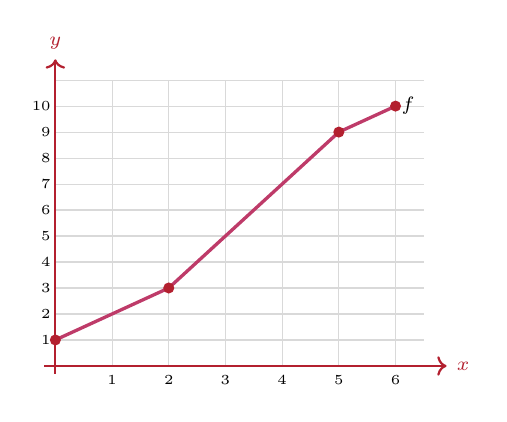
\begin{tikzpicture}[x=0.72cm,y=0.33cm]
\draw[gray!30,xstep=1,ystep=1] (0,0) grid (6.5,11);
\draw[->,thick,redx] (-0.2,0)--(6.9,0) node[right,font=\scriptsize]{$x$};
\draw[->,thick,redx] (0,-0.3)--(0,11.8) node[above,font=\scriptsize]{$y$};
\foreach \xx in {1,2,3,4,5,6}{\node[below,font=\tiny] at (\xx,0) {\xx};}
\foreach \yy in {1,2,3,4,5,6,7,8,9,10}{\node[left,font=\tiny,inner sep=1.5pt] at (0,\yy) {\yy};}
\draw[pinkx!85!black,very thick] (0,1)--(2,3)--(5,9)--(6,10);
\foreach \px/\py in {0/1,2/3,5/9,6/10}{\fill[redx] (\px,\py) circle (2pt);}
\node[font=\scriptsize,right,inner sep=2pt] at (6,10) {$f$};
\end{tikzpicture}}}{\pil{$2$}{$4$}{$5$}{$6$}{$8$}}
\soal{Diketahui $f(x)=x^2-4x+7$ dan $g(x)=\dis\frac{1}{\sqrt{x-a}}$ dengan $a$ bilangan real. Jika $(g\circ f)(x)$ terdefinisi untuk setiap bilangan real $x$, himpunan semua nilai $a$ yang memenuhi adalah \dots.}{\pil{$a>3$}{$a\ge3$}{$a\le3$}{$a<7$}{$a<3$}}
\soal{Diketahui $f(x)=ax+b$ dan $g(x)=x+2$ dengan $a\neq0$. Apakah $(f\circ g)(x)=(g\circ f)(x)$ untuk setiap bilangan real $x$?
\begin{enumerate}[label=(\arabic*),leftmargin=1.8em,itemsep=0pt,topsep=2pt]
\item $f(3)-f(1)=2$.
\item $f(0)=5$.
\end{enumerate}}{\begin{tabularx}{\linewidth}{@{}lX@{}}
\textbf{A.} & Pernyataan (1) SAJA cukup untuk menjawab pertanyaan, tetapi pernyataan (2) SAJA tidak cukup.\\
\textbf{B.} & Pernyataan (2) SAJA cukup untuk menjawab pertanyaan, tetapi pernyataan (1) SAJA tidak cukup.\\
\textbf{C.} & DUA pernyataan BERSAMA-SAMA cukup untuk menjawab pertanyaan, tetapi SATU pernyataan SAJA tidak cukup.\\
\textbf{D.} & Pernyataan (1) SAJA cukup dan pernyataan (2) SAJA cukup untuk menjawab pertanyaan.\\
\textbf{E.} & Pernyataan (1) dan pernyataan (2) tidak cukup untuk menjawab pertanyaan.
\end{tabularx}}

% =====================================================================
\bagian{B. Isian Singkat}{5 soal $\times$ 4 poin = 20 poin. Tuliskan hanya jawaban akhir.}

\tingkat{Tingkat Mudah dan Sedang}{soal 1 dan 2}
\soal{Diketahui $f(x)=2x-3$ dan $g(x)=x^2+1$. Nilai $(f\circ g)(3)+(g\circ f)(3)$ adalah \dots}{\jwb}
\soal{Sebuah rangkaian dua mesin bekerja seperti pada gambar. Mesin $f$ menerima masukan $x>0$, hasilnya diteruskan ke mesin $g$, dan keluaran akhirnya adalah $120$. Nilai $x$ adalah \dots
\begin{center}
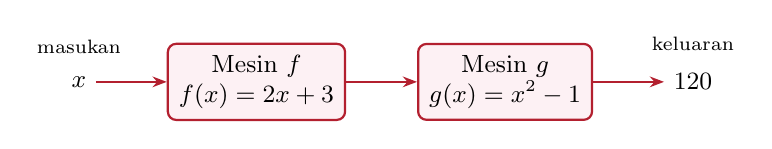
\begin{tikzpicture}[font=\small]
\node (in) {$x$};
\node[box,right=0.9cm of in] (m1) {Mesin $f$\\$f(x)=2x+3$};
\node[box,right=0.9cm of m1] (m2) {Mesin $g$\\$g(x)=x^2-1$};
\node[right=0.9cm of m2] (out) {$120$};
\draw[ar] (in)--(m1); \draw[ar] (m1)--(m2); \draw[ar] (m2)--(out);
\node[font=\scriptsize,above=0.05cm of in] {masukan};
\node[font=\scriptsize,above=0.05cm of out] {keluaran};
\end{tikzpicture}
\end{center}}{\jwb}

\tingkat{Tingkat Sulit}{soal 3 dan 4}
\soal{Diketahui $f(x)=x+2$ dan $(g\circ f)(x)=\dis\frac{3x+5}{x+1}$, $x\neq-1$. Nilai $g^{-1}(5)$ adalah \dots}{\jwb}
\soal{\gbr{Gambar menunjukkan grafik fungsi $f(x)=a\cdot2^{x}+b$ yang melalui titik $(0,3)$ dan $(2,6)$. Jika $f^{-1}$ adalah invers dari $f$, nilai $f^{-1}(18)$ adalah \dots}{%
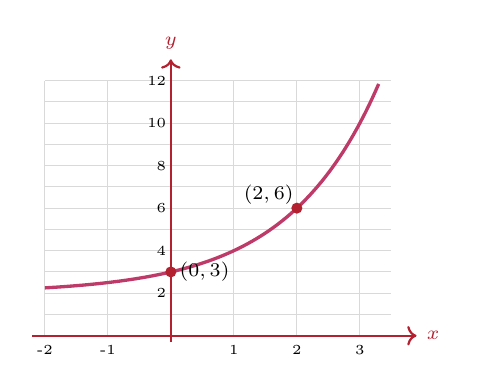
\begin{tikzpicture}[x=0.8cm,y=0.27cm]
\draw[gray!30,xstep=1,ystep=1] (-2,0) grid (3.5,12);
\draw[->,thick,redx] (-2.2,0)--(3.9,0) node[right,font=\scriptsize]{$x$};
\draw[->,thick,redx] (0,-0.3)--(0,13) node[above,font=\scriptsize]{$y$};
\foreach \xx in {-2,-1,1,2,3}{\node[below,font=\tiny] at (\xx,0) {\xx};}
\foreach \yy in {2,4,6,8,10,12}{\node[left,font=\tiny,inner sep=1.5pt] at (0,\yy) {\yy};}
\draw[pinkx!85!black,very thick,domain=-2:3.3,samples=50,smooth] plot (\x,{2^(\x)+2});
\fill[redx] (0,3) circle (2pt) (2,6) circle (2pt);
\node[font=\scriptsize,right,inner sep=3pt] at (0,3) {$(0,3)$};
\node[font=\scriptsize,above left,inner sep=1pt] at (2,6) {$(2,6)$};
\end{tikzpicture}}}{\jwb}

\tingkat{Tingkat HOTS}{soal 5}
\soal{\gbr{Gambar menunjukkan grafik fungsi $f(x)=x^2-4x+6$ dengan domain $\{x\mid x\ge2\}$, grafik inversnya $f^{-1}$, dan garis $y=x$. Kedua grafik berpotongan di titik $A$ dan titik $B$. Panjang ruas garis $AB$ adalah \dots}{%
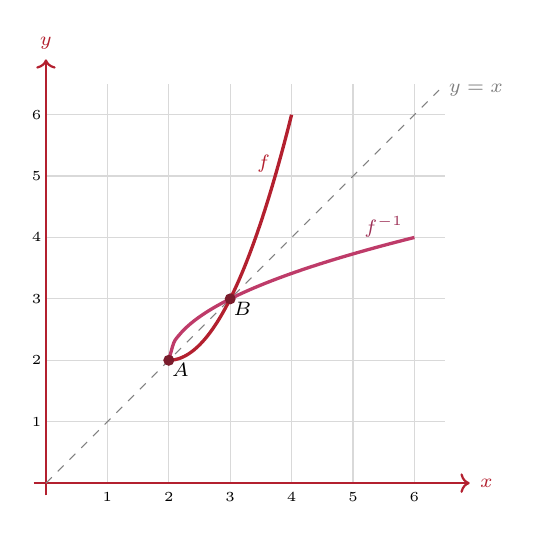
\begin{tikzpicture}[x=0.78cm,y=0.78cm]
\draw[gray!30,xstep=1,ystep=1] (0,0) grid (6.5,6.5);
\draw[->,thick,redx] (-0.2,0)--(6.9,0) node[right,font=\scriptsize]{$x$};
\draw[->,thick,redx] (0,-0.2)--(0,6.9) node[above,font=\scriptsize]{$y$};
\foreach \xx in {1,2,3,4,5,6}{\node[below,font=\tiny] at (\xx,0) {\xx};}
\foreach \yy in {1,2,3,4,5,6}{\node[left,font=\tiny,inner sep=1.5pt] at (0,\yy) {\yy};}
\draw[gray,dashed] (0,0)--(6.4,6.4) node[right,font=\scriptsize]{$y=x$};
\draw[redx,very thick,domain=2:4,samples=40,smooth] plot (\x,{\x*\x-4*\x+6});
\draw[pinkx!85!black,very thick,domain=2:6,samples=50,smooth] plot (\x,{2+sqrt(\x-2)});
\fill[maroon] (2,2) circle (2pt) (3,3) circle (2pt);
\node[font=\scriptsize,below right,inner sep=1pt] at (2,2) {$A$};
\node[font=\scriptsize,below right,inner sep=1pt] at (3,3) {$B$};
\node[font=\scriptsize,redx,left,inner sep=2pt] at (3.75,5.2) {$f$};
\node[font=\scriptsize,pinkx!70!black,above,inner sep=2pt] at (5.5,3.9) {$f^{-1}$};
\end{tikzpicture}}}{\jwb}

% =====================================================================
\bagian{C. Uraian (Essay)}{5 soal $\times$ 8 poin = 40 poin. Tuliskan langkah penyelesaian dengan lengkap.}

\tingkat{Tingkat Sedang}{soal 1 dan 2}
\soal{Diketahui $f(x)=2x+3$ dan $g(x)=x^2-4x$.\par\smallskip
(a) Tentukan rumus $(f\circ g)(x)$ dan $(g\circ f)(x)$.\par
(b) Hitunglah $(f\circ g)(5)$ dan $(g\circ f)(-2)$.\par
(c) Tentukan semua nilai $x$ yang memenuhi $(f\circ g)(x)=3$.\par
(d) Apakah $f\circ g=g\circ f$? Buktikan jawabanmu dengan satu nilai $x$ sebagai contoh.}{\poin{8}}
\soal{\gbr{Gambar menunjukkan grafik fungsi $f(x)=\dis\frac{2x-1}{x+4}$.\par\smallskip(a) Dari gambar, tentukan persamaan asimtot tegak dan asimtot datar, lalu tuliskan domain dan range $f$.\par(b) Tentukan rumus $f^{-1}(x)$ beserta domain dan range-nya.\par(c) Hitunglah $f^{-1}(3)$.\par(d) Buktikan bahwa $f\big(f^{-1}(x)\big)=x$.}{%
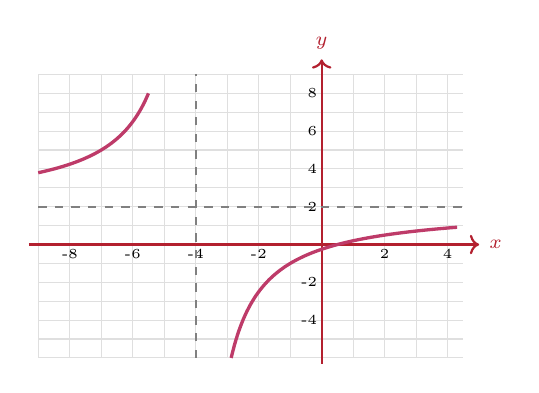
\begin{tikzpicture}[x=0.4cm,y=0.24cm]
\draw[gray!25,xstep=1,ystep=1] (-9,-6) grid (4.5,9);
\draw[->,thick,redx] (-9.3,0)--(5,0) node[right,font=\scriptsize]{$x$};
\draw[->,thick,redx] (0,-6.3)--(0,9.8) node[above,font=\scriptsize]{$y$};
\foreach \xx in {-8,-6,-4,-2,2,4}{\node[below,font=\tiny,inner sep=1.5pt] at (\xx,0) {\xx};}
\foreach \yy in {-4,-2,2,4,6,8}{\node[left,font=\tiny,inner sep=1.5pt] at (0,\yy) {\yy};}
\draw[gray,dashed,thick] (-4,-6)--(-4,9);
\draw[gray,dashed,thick] (-9,2)--(4.5,2);
\draw[pinkx!85!black,very thick,domain=-9:-5.5,samples=40,smooth] plot (\x,{2-9/(\x+4)});
\draw[pinkx!85!black,very thick,domain=-2.875:4.3,samples=60,smooth] plot (\x,{2-9/(\x+4)});
\end{tikzpicture}}}{\poin{8}}

\Needspace{24\baselineskip}
\tingkat{Tingkat Sulit}{soal 3 dan 4}
\soal{Diagram panah berikut menunjukkan fungsi $f:A\to B$ dan $g:B\to C$ dengan $A=\{1,2,3,4\}$, $B=\{2,4,6,8\}$, dan $C=\{5,7,9,11\}$.
\begin{center}
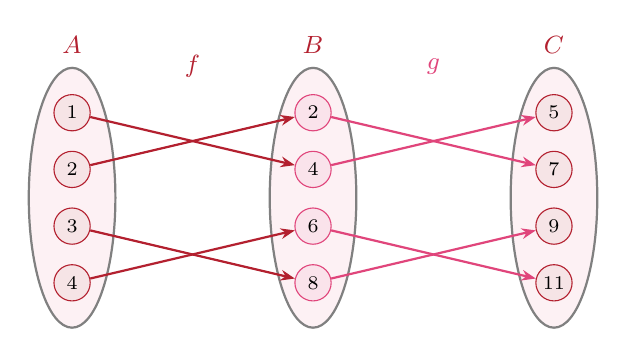
\begin{tikzpicture}[scale=0.9]
\node[font=\small\bfseries,redx] at (0,2.15) {$A$};
\node[font=\small\bfseries,redx] at (3.4,2.15) {$B$};
\node[font=\small\bfseries,redx] at (6.8,2.15) {$C$};
\node[ov,minimum width=1.1cm,minimum height=3.3cm] at (0,0) {};
\node[ov,minimum width=1.1cm,minimum height=3.3cm] at (3.4,0) {};
\node[ov,minimum width=1.1cm,minimum height=3.3cm] at (6.8,0) {};
\foreach \yy/\l in {1.2/1,0.4/2,-0.4/3,-1.2/4}{\node[dr] (a\l) at (0,\yy) {\l};}
\foreach \yy/\l/\v in {1.2/1/2,0.4/2/4,-0.4/3/6,-1.2/4/8}{\node[dk] (b\l) at (3.4,\yy) {\v};}
\foreach \yy/\l/\v in {1.2/1/5,0.4/2/7,-0.4/3/9,-1.2/4/11}{\node[dr] (c\l) at (6.8,\yy) {\v};}
\foreach \i/\j in {1/2,2/1,3/4,4/3}{\draw[ar] (a\i)--(b\j);}
\foreach \i/\j in {1/2,2/1,3/4,4/3}{\draw[arp] (b\i)--(c\j);}
\node[font=\small,redx] at (1.7,1.85) {$f$};
\node[font=\small,pinkx] at (5.1,1.85) {$g$};
\end{tikzpicture}
\end{center}
(a) Tuliskan $g\circ f$ sebagai himpunan pasangan berurutan, lalu tentukan rumus $(g\circ f)(x)$.\par
(b) Selidiki apakah $f$, $g$, dan $g\circ f$ masing-masing merupakan fungsi bijektif. Berikan alasan.\par
(c) Tuliskan $f^{-1}$ dan $g^{-1}$ sebagai himpunan pasangan berurutan.\par
(d) Tentukan $(g\circ f)^{-1}(9)$ dengan dua cara: melalui $f^{-1}\circ g^{-1}$ dan melalui rumus $(g\circ f)^{-1}(x)$. Mengapa urutan $f^{-1}$ dan $g^{-1}$ tertukar?}{\poin{8}}
\soal{Sebuah pabrik tepung memproses bahan baku melalui tiga mesin berurutan. Mesin I mengubah $x$ ton gandum menjadi $f(x)=0{,}8x$ ton tepung kasar. Mesin II mengayak $y$ ton tepung kasar menjadi $g(y)=0{,}75y-0{,}5$ ton tepung halus (ada $0{,}5$ ton yang tertinggal di mesin). Mesin III mengemas $z$ ton tepung halus menjadi $h(z)=50z$ kemasan.
\begin{center}
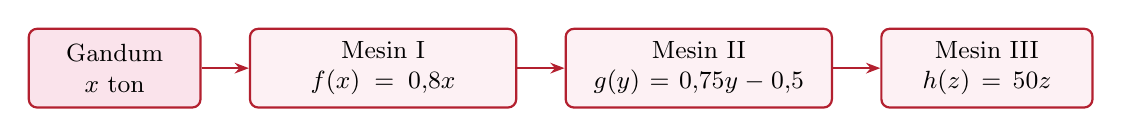
\begin{tikzpicture}[font=\small,bx/.style={box,text width=3.1cm,minimum height=1.0cm}]
\node[bx,fill=pinkx!15,text width=1.9cm] (a) {Gandum\\$x$ ton};
\node[bx,right=0.6cm of a] (b) {Mesin I\\$f(x)=0{,}8x$};
\node[bx,right=0.6cm of b] (c) {Mesin II\\$g(y)=0{,}75y-0{,}5$};
\node[bx,right=0.6cm of c,text width=2.4cm] (d) {Mesin III\\$h(z)=50z$};
\foreach \p/\q in {a/b,b/c,c/d}{\draw[ar] (\p)--(\q);}
\end{tikzpicture}
\end{center}
(a) Tentukan fungsi total $T(x)=(h\circ g\circ f)(x)$, yaitu banyak kemasan dari $x$ ton gandum.\par
(b) Berapa kemasan yang dihasilkan dari $80$ ton gandum?\par
(c) Tentukan $T^{-1}(x)$, lalu hitung banyak gandum yang diperlukan untuk memenuhi pesanan $1.475$ kemasan.\par
(d) Tentukan batas minimum $x$ agar $T(x)\ge0$, lalu jelaskan arti batas tersebut pada mesin II.}{\poin{8}}

\tingkat{Tingkat HOTS}{soal 5}
\soal{Diketahui $f(x)=\dis\frac{2x+5}{x-2}$, $x\neq2$, dan $g(x)=3x-1$.\par\smallskip
(a) Buktikan bahwa $f\big(f(x)\big)=x$ untuk setiap $x\neq2$ dalam domain komposisinya, sehingga $f^{-1}=f$.\par
(b) Jika $f^{(n)}$ menyatakan komposisi $f$ sebanyak $n$ kali, tentukan $f^{(2027)}(3)$ dengan memanfaatkan hasil (a).\par
(c) Tentukan $(f\circ g)^{-1}(x)$ dengan dua cara: melalui rumus $(f\circ g)(x)$ dan melalui $g^{-1}\circ f^{-1}$. Pastikan kedua hasilnya sama.\par
(d) Tentukan semua nilai $x$ yang memenuhi $(f\circ g)^{-1}(x)=(f\circ g)(x)$.}{\poin{8}}

% =====================================================================
\newpage
\bagian{Kunci Jawaban dan Pembahasan Singkat}{Untuk guru dan pembahasan mandiri}
\par\vspace{0.6em}{\bfseries\color{redx}Kunci Pilihan Ganda}\par\vspace{0.3em}
\small
\begin{tabularx}{\linewidth}{@{}*{10}{>{\centering\arraybackslash}X}@{}}\hline \textbf{1} & \textbf{2} & \textbf{3} & \textbf{4} & \textbf{5} & \textbf{6} & \textbf{7} & \textbf{8} & \textbf{9} & \textbf{10}\\ \hline D & B & C & A & E & C & B & A & D & E\\ \hline\end{tabularx}\\[6pt]
\begin{tabularx}{\linewidth}{@{}*{10}{>{\centering\arraybackslash}X}@{}}\hline \textbf{11} & \textbf{12} & \textbf{13} & \textbf{14} & \textbf{15} & \textbf{16} & \textbf{17} & \textbf{18} & \textbf{19} & \textbf{20}\\ \hline C & D & B & A & C & E & B & D & E & A\\ \hline\end{tabularx}
\par\vspace{0.8em}{\bfseries\color{redx}\normalsize Pembahasan Pilihan Ganda}\par\vspace{0.2em}
\small\begin{enumerate}[leftmargin=2em,itemsep=2pt,topsep=2pt]
\item[\textbf{1.}] \textbf{(D)} $f(2)=3\cdot2-2=4$, lalu $g(4)=4^2+1=17$. (Jebakan: $(f\circ g)(2)=f(5)=13$ karena urutan tertukar.)
\item[\textbf{2.}] \textbf{(B)} $g\circ f$ memetakan $1\to3\to10$, $2\to5\to20$, $3\to5\to20$, $4\to7\to30$. Jadi $R_{g\circ f}=\{10,20,30\}$. Angka $40$ tidak masuk range karena $9$ bukan hasil dari $f$.
\item[\textbf{3.}] \textbf{(C)} Dari $y=3x-6$ diperoleh $x=\dis\frac{y+6}{3}$, sehingga $f^{-1}(9)=\dis\frac{15}{3}=5$. Cara cepat: selesaikan $3x-6=9$, hasilnya $x=5$.
\item[\textbf{4.}] \textbf{(A)} $(f\circ g)(2)=f(g(2))=f(1)=3$ dan $(g\circ f)(4)=g(f(4))=g(2)=1$, sehingga jumlahnya $4$. (Jebakan: jika urutan dibalik, $(g\circ f)(2)+(f\circ g)(4)=4+4=8$.)
\item[\textbf{5.}] \textbf{(E)} $(g\circ f)(x)=g(x+2)=3(x+2)-1=3x+5$. (Jawaban $3x+1$ adalah $(f\circ g)(x)$.)
\item[\textbf{6.}] \textbf{(C)} $(f\circ g)(x)=2g(x)+1=6x-5\Rightarrow g(x)=\dis\frac{6x-6}{2}=3x-3$.
\item[\textbf{7.}] \textbf{(B)} Karena $g(x)=5$ dicapai saat $x=7$, maka $f(5)=(f\circ g)(7)=49-28+5=26$. Cara lain: $x^2-4x+5=(x-2)^2+1$, sehingga $f(t)=t^2+1$ dan $f(5)=26$. (Jebakan $10$: memakai $(f\circ g)(5)$.)
\item[\textbf{8.}] \textbf{(A)} Dari $y=\dis\frac{3x-1}{x+2}$ diperoleh $xy+2y=3x-1\Rightarrow x(y-3)=-2y-1\Rightarrow x=\dis\frac{2y+1}{3-y}$. Jadi $f^{-1}(x)=\dis\frac{2x+1}{3-x}$. Rumus cepat: $\dis\frac{ax+b}{cx+d}\Rightarrow\dis\frac{-dx+b}{cx-a}=\dis\frac{-2x-1}{x-3}$.
\item[\textbf{9.}] \textbf{(D)} Gradien $=\dis\frac{3-(-1)}{3-1}=2$, sehingga $y+1=2(x-1)$ atau $f(x)=2x-3$. Maka $f^{-1}(7)$ memenuhi $2x-3=7$, yaitu $x=5$. (Jebakan $2$: salah memakai $\frac{x-3}{2}$.)
\item[\textbf{10.}] \textbf{(E)} $(f\circ g)(x)=\sqrt{x^2-4x+3}$ terdefinisi jika $x^2-4x+3\ge0$, yaitu $(x-1)(x-3)\ge0$, sehingga $x\le1$ atau $x\ge3$. (Jawaban A adalah penyelesaian untuk $\le0$.)
\item[\textbf{11.}] \textbf{(C)} $(f\circ g)(x)=2\cdot\dis\frac{x+1}{x-2}-3=\dis\frac{8-x}{x-2}$. Nilai $(f\circ g)^{-1}(3)$ adalah $x$ yang memenuhi $\dis\frac{8-x}{x-2}=3\Rightarrow8-x=3x-6\Rightarrow x=\dis\frac72$. Cara lain: $(f\circ g)^{-1}=g^{-1}\circ f^{-1}$, dengan urutan invers dibalik.
\item[\textbf{12.}] \textbf{(D)} Selesaikan $x^2-4x+1=6\Rightarrow x^2-4x-5=0\Rightarrow(x-5)(x+1)=0$. Domain $x\ge2$ sehingga hanya $x=5$ yang berlaku. (Jebakan $-1$: berada di cabang kiri parabola yang tidak termasuk domain.)
\item[\textbf{13.}] \textbf{(B)} $(f\circ f)(x)=a(ax+b)+b=a^2x+(a+1)b$. Maka $a^2=4$ dan $a>0$ memberi $a=2$, lalu $3b=9\Rightarrow b=3$. Jadi $f(x)=2x+3$ dan $f^{-1}(11)$ memenuhi $2x+3=11$, yaitu $x=4$. (Tanpa syarat $a>0$ ada pasangan lain $a=-2,b=-9$.)
\item[\textbf{14.}] \textbf{(A)} (1) $g(f(x))=2(x^2-1)+1=2x^2-1$, \emph{benar}. (2) $f(g(x))=(2x+1)^2-1=4x^2+4x$, \emph{benar}. (3) $f(1)=f(-1)=0$, jadi $f$ tidak satu-satu dan tidak punya invers pada $\mathbb{R}$, \emph{benar}. (4) $f(2)=3$ dan $g^{-1}(x)=\dis\frac{x-1}{2}$, sehingga $g^{-1}(3)=1\neq2$, \emph{salah}.
\item[\textbf{15.}] \textbf{(C)} Urutan: voucher, diskon, lalu PPN, yaitu $h\big(f(g(x))\big)=1{,}1\cdot0{,}8\,(x-20.000)=0{,}88\,(x-20.000)=132.000$. Maka $x-20.000=150.000$ dan $x=170.000$. (Jebakan D: jika diskon dihitung lebih dulu sebelum voucher, hasilnya $175.000$.)
\item[\textbf{16.}] \textbf{(E)} $f\big(f(x)\big)=\dis\frac{\frac{x+1}{x-1}+1}{\frac{x+1}{x-1}-1}=\dis\frac{2x}{2}=x$, sehingga $f$ adalah invers dirinya sendiri dan komposisi genap menghasilkan fungsi identitas. Karena $2027$ ganjil, $f^{(2027)}=f$, dan $f\!\left(\frac32\right)=\dis\frac{5/2}{1/2}=5$. (Jebakan $\frac32$: menganggap hasilnya kembali ke nilai awal.)
\item[\textbf{17.}] \textbf{(B)} Untuk $f(x)=\dis\frac{ax+b}{cx+d}$, syarat $f^{-1}=f$ adalah $d=-a$. Di sini $d=-3$, sehingga $a=3$. Lalu $f(2)=\dis\frac{6+b}{4-3}=6+b=5\Rightarrow b=-1$. Jadi $a+b=2$. (Cek: $f^{-1}(x)=\dis\frac{3x-1}{2x-3}=f(x)$.)
\item[\textbf{18.}] \textbf{(D)} Ruas pertama $f(x)=x+1$ sehingga $f(1)=2$ dan $f(2)=3$, jadi $(f\circ f)(1)=3$. Dari grafik $f(5)=9$, sehingga $f^{-1}(9)=5$. Pada ruas kedua $f(x)=2x-1$, dan $2x-1=5\Rightarrow x=3$, sehingga $f^{-1}(5)=3$. Jadi $(f^{-1}\circ f^{-1})(9)=3$ dan jumlahnya $3+3=6$.
\item[\textbf{19.}] \textbf{(E)} $f(x)=(x-2)^2+3\ge3$ sehingga $R_f=[3,\infty)$. Fungsi $g$ terdefinisi hanya jika $x-a>0$, jadi harus $f(x)>a$ untuk semua $x$, yaitu $3>a$. Nilai $a=3$ tidak boleh karena $f(2)=3$ membuat penyebut $\sqrt{0}=0$.
\item[\textbf{20.}] \textbf{(A)} $(f\circ g)(x)=a(x+2)+b=ax+2a+b$ dan $(g\circ f)(x)=ax+b+2$. Keduanya sama untuk semua $x$ jika dan hanya jika $2a=2$, yaitu $a=1$ (nilai $b$ tidak berpengaruh). Pernyataan (1): $f(3)-f(1)=2a=2\Rightarrow a=1$, cukup. Pernyataan (2) hanya memberi $b=5$ tanpa informasi $a$, tidak cukup.
\end{enumerate}
\par\Needspace{6\baselineskip}\vspace{0.6em}{\bfseries\color{redx}\normalsize Pembahasan Isian Singkat}\par\vspace{0.2em}
\small\begin{enumerate}[leftmargin=2em,itemsep=2pt,topsep=2pt]
\item[\textbf{1.}] \textbf{Jawaban: $27$.} $(f\circ g)(3)=f(10)=17$ dan $(g\circ f)(3)=g(3)=10$. Jumlahnya $27$.
\item[\textbf{2.}] \textbf{Jawaban: $4$.} $g\big(f(x)\big)=(2x+3)^2-1=120\Rightarrow(2x+3)^2=121\Rightarrow2x+3=\pm11$. Karena $x>0$, $2x+3=11$ sehingga $x=4$ (nilai $x=-7$ ditolak).
\item[\textbf{3.}] \textbf{Jawaban: $2$.} Misalkan $t=x+2$, maka $g(t)=\dis\frac{3(t-2)+5}{(t-2)+1}=\dis\frac{3t-1}{t-1}$. Nilai $g^{-1}(5)$ memenuhi $\dis\frac{3t-1}{t-1}=5\Rightarrow3t-1=5t-5\Rightarrow t=2$.
\item[\textbf{4.}] \textbf{Jawaban: $4$.} Dari titik $(0,3)$: $a+b=3$. Dari titik $(2,6)$: $4a+b=6$. Maka $a=1$ dan $b=2$, sehingga $f(x)=2^x+2$. Selesaikan $2^x+2=18\Rightarrow2^x=16\Rightarrow x=4$.
\item[\textbf{5.}] \textbf{Jawaban: $\sqrt{2}$.} Pada domain $x\ge2$, $f$ naik, sehingga titik potong $f$ dan $f^{-1}$ terletak pada garis $y=x$. Selesaikan $x^2-4x+6=x\Rightarrow x^2-5x+6=0\Rightarrow x=2$ atau $x=3$. Titik potongnya $A(2,2)$ dan $B(3,3)$, sehingga $AB=\sqrt{1^2+1^2}=\sqrt2$.
\end{enumerate}
\par\Needspace{8\baselineskip}\vspace{0.6em}{\bfseries\color{redx}\normalsize Pembahasan dan Pedoman Penskoran Uraian}\par\vspace{0.2em}
\small\begin{enumerate}[leftmargin=2em,itemsep=3pt,topsep=2pt]
\item[\textbf{1.}] (a) $(f\circ g)(x)=2(x^2-4x)+3=2x^2-8x+3$. $(g\circ f)(x)=(2x+3)^2-4(2x+3)=4x^2+12x+9-8x-12=4x^2+4x-3$. (b) $(f\circ g)(5)=50-40+3=13$. $f(-2)=-1$ dan $g(-1)=1+4=5$, sehingga $(g\circ f)(-2)=5$. (c) $2x^2-8x+3=3\Rightarrow2x(x-4)=0\Rightarrow x=0$ atau $x=4$. (d) Tidak. Untuk $x=1$: $(f\circ g)(1)=2-8+3=-3$, sedangkan $(g\circ f)(1)=4+4-3=5$. Karena hasilnya berbeda, $f\circ g\neq g\circ f$ (komposisi tidak komutatif). \\ \textit{Penskoran: (a) 2 poin; (b) 2 poin; (c) 2 poin; (d) 2 poin.}
\item[\textbf{2.}] (a) Asimtot tegak $x=-4$ dan asimtot datar $y=2$. $D_f=\{x\mid x\neq-4\}$ dan $R_f=\{y\mid y\neq2\}$. (b) $y=\dis\frac{2x-1}{x+4}\Rightarrow xy+4y=2x-1\Rightarrow x(y-2)=-4y-1\Rightarrow x=\dis\frac{4y+1}{2-y}$. Jadi $f^{-1}(x)=\dis\frac{4x+1}{2-x}$ dengan domain $\{x\mid x\neq2\}$ dan range $\{y\mid y\neq-4\}$ (domain dan range tertukar). (c) $f^{-1}(3)=\dis\frac{13}{2-3}=-13$. Cek: $f(-13)=\dis\frac{-27}{-9}=3$. (d) $f\big(f^{-1}(x)\big)=\dis\frac{2\cdot\frac{4x+1}{2-x}-1}{\frac{4x+1}{2-x}+4}=\dis\frac{\frac{8x+2-2+x}{2-x}}{\frac{4x+1+8-4x}{2-x}}=\dis\frac{9x}{9}=x$. \\ \textit{Penskoran: (a) 2 poin (asimtot 1, domain dan range 1); (b) 2 poin; (c) 2 poin; (d) 2 poin.}
\item[\textbf{3.}] (a) $g\circ f=\{(1,5),(2,7),(3,9),(4,11)\}$. Pola $x\mapsto2x+3$, sehingga $(g\circ f)(x)=2x+3$. (b) $f$ bijektif karena setiap anggota $B$ tepat sekali menjadi pasangan anggota $A$ (satu-satu dan pada). $g$ bijektif dengan alasan yang sama terhadap $C$. $g\circ f$ memetakan empat anggota $A$ ke empat anggota $C$ yang berbeda dan semuanya terpakai, sehingga bijektif. (c) $f^{-1}=\{(4,1),(2,2),(8,3),(6,4)\}$ dan $g^{-1}=\{(7,2),(5,4),(11,6),(9,8)\}$. (d) Cara 1: $g^{-1}(9)=8$, lalu $f^{-1}(8)=3$. Cara 2: $(g\circ f)^{-1}(x)=\dis\frac{x-3}{2}$, sehingga $(g\circ f)^{-1}(9)=3$. Urutan tertukar karena $g\circ f$ menerapkan $f$ lebih dulu; untuk membalikkannya, yang terakhir diterapkan ($g$) harus dibalik lebih dulu, yaitu $(g\circ f)^{-1}=f^{-1}\circ g^{-1}$. \\ \textit{Penskoran: (a) 2 poin (pasangan 1, rumus 1); (b) 2 poin; (c) 2 poin; (d) 2 poin.}
\item[\textbf{4.}] (a) $T(x)=50\big(0{,}75\cdot0{,}8x-0{,}5\big)=50(0{,}6x-0{,}5)=30x-25$. (b) $T(80)=2400-25=2375$ kemasan. (c) Dari $y=30x-25$ diperoleh $x=\dis\frac{y+25}{30}$, sehingga $T^{-1}(x)=\dis\frac{x+25}{30}$. Untuk pesanan $1.475$ kemasan: $T^{-1}(1475)=\dis\frac{1500}{30}=50$ ton gandum. (d) $30x-25\ge0\Rightarrow x\ge\dis\frac56$ ton. Pada batas ini tepung kasar yang masuk ke mesin II adalah $0{,}8\cdot\dis\frac56=\dis\frac23$ ton, dan $g\!\left(\dis\frac23\right)=0$. Jika gandum kurang dari $\dis\frac56$ ton, seluruh tepung habis tertinggal di mesin II dan hasil negatif tidak bermakna. \\ \textit{Penskoran: (a) 2 poin; (b) 2 poin; (c) 2 poin (invers 1, nilai 1); (d) 2 poin.}
\item[\textbf{5.}] (a) $f\big(f(x)\big)=\dis\frac{2\cdot\frac{2x+5}{x-2}+5}{\frac{2x+5}{x-2}-2}=\dis\frac{\frac{4x+10+5x-10}{x-2}}{\frac{2x+5-2x+4}{x-2}}=\dis\frac{9x}{9}=x$. Karena $f\circ f$ adalah fungsi identitas, $f^{-1}=f$. (b) $f^{(2)}=I$ sehingga $f^{(2026)}=I$ dan $f^{(2027)}=f$. Maka $f^{(2027)}(3)=f(3)=\dis\frac{11}{1}=11$. (c) Cara 1: $(f\circ g)(x)=\dis\frac{2(3x-1)+5}{(3x-1)-2}=\dis\frac{6x+3}{3x-3}=\dis\frac{2x+1}{x-1}$. Dari $y=\dis\frac{2x+1}{x-1}$ diperoleh $x(y-2)=y+1$, sehingga $(f\circ g)^{-1}(x)=\dis\frac{x+1}{x-2}$. Cara 2: $g^{-1}(x)=\dis\frac{x+1}{3}$ dan $f^{-1}=f$, sehingga $g^{-1}\big(f(x)\big)=\dis\frac{\frac{2x+5}{x-2}+1}{3}=\dis\frac{3x+3}{3(x-2)}=\dis\frac{x+1}{x-2}$. Kedua hasil sama. (d) $\dis\frac{x+1}{x-2}=\dis\frac{2x+1}{x-1}\Rightarrow(x+1)(x-1)=(2x+1)(x-2)\Rightarrow x^2-1=2x^2-3x-2\Rightarrow x^2-3x-1=0$. Maka $x=\dis\frac{3\pm\sqrt{13}}{2}$. Kedua nilai tidak sama dengan $1$ atau $2$, sehingga keduanya memenuhi. \\ \textit{Penskoran: (a) 2 poin; (b) 2 poin; (c) 2 poin (dua cara masing-masing 1); (d) 2 poin.}
\end{enumerate}
\end{document}
